\documentclass[11pt, a4paper]{article}
\usepackage[a4paper, total={6.5 in,9in}]{geometry}
\usepackage[slovene]{babel}
\usepackage[utf8]{inputenc}
\usepackage[T1]{fontenc}
\usepackage{lmodern}
\usepackage{amsmath}
\usepackage{ amssymb }
\usepackage{amsfonts}
\usepackage{amsthm}
\usepackage{comment}
\usepackage{url}
\usepackage{gensymb}
\usepackage{subcaption}
\usepackage[pdftex]{graphicx}
\usepackage[section]{placeins}
\usepackage{mathtools}
\usepackage{float}
\usepackage{epstopdf}
\renewcommand{\vec}[1]{\mathbf{#1}}
\usepackage{hyperref}
\usepackage{wrapfig}

\pagestyle{plain}

\begin{document}

    \begin{center}
    {\LARGE\bfseries 8. Generatorji naključnih števil \par}
    \vspace{1cm}
    
    {\Large Domača naloga pri predmetu Modelska analiza I\par}
    \vspace{0.2cm}
    {\normalsize Avtor: Matic Noč \par}
    \vspace{0.2cm}    
    {\normalsize 15.11.2017 \par}    

    
    \end{center}
\section{Uvod}
Obravnavamo generatorje naključnih števil. Naključna števila bodo pri dobrem generatorju vedno porazdeljena enakomerno. Ker pa potrebujemo naključna števila tudi v različnih porazdelitvah, geometrijskih oblikah, lahko s transformacijami dveh naključnih števil izračunamo nova naključna števila, ki so drugače porazdeljena. Ogledali si bomo različno porazdeljena naključna števila, preverili njihove porazdelitve s statističnimi testi in nato obravnavali statistično analizo oddaje nalog modelske analize.


\section{Generator naključnih števil}
Preverimo najprej delovanje generatorja naključnih števil. Uporabili bomo pseudorandom Mersenne Tvister (1997 by Makoto Matsumoto in Nishimura), ki ima periodo  $2^{19937} - 1$ in serijsko enakomernost do 623 števil.
\subsection{Enakomerna porazdelitev naključnih števil}
Če računamo naključna števila med 0 in 1 moramo dobiti enakomerno porazdelitev števil. Poglejmo si histograme in statistične teste generatorja Marsenne Twister. Najprej testiramo s $chi^2$ statistiko: 
\begin{equation}
\chi^2 = \sum_i^n \frac{(O_i-E_i)^2}{E_i^2}
\end{equation}
kjer je i parameter razreda, O izmerjeno/zaznano število spremenljivke v določenem razredu in E pričakovano število spremenljivke v i-tem razredu. V primeru enakomerne porazdelitve je $E_i = \int_{x_{i}}^{x_{i+1}} \frac{dP}{dx} dx = \bf{\frac{1}{n} N}$, kjer je N število vseh izmerkov.
\begin{figure}[H]
\hspace*{-2.5cm}  
  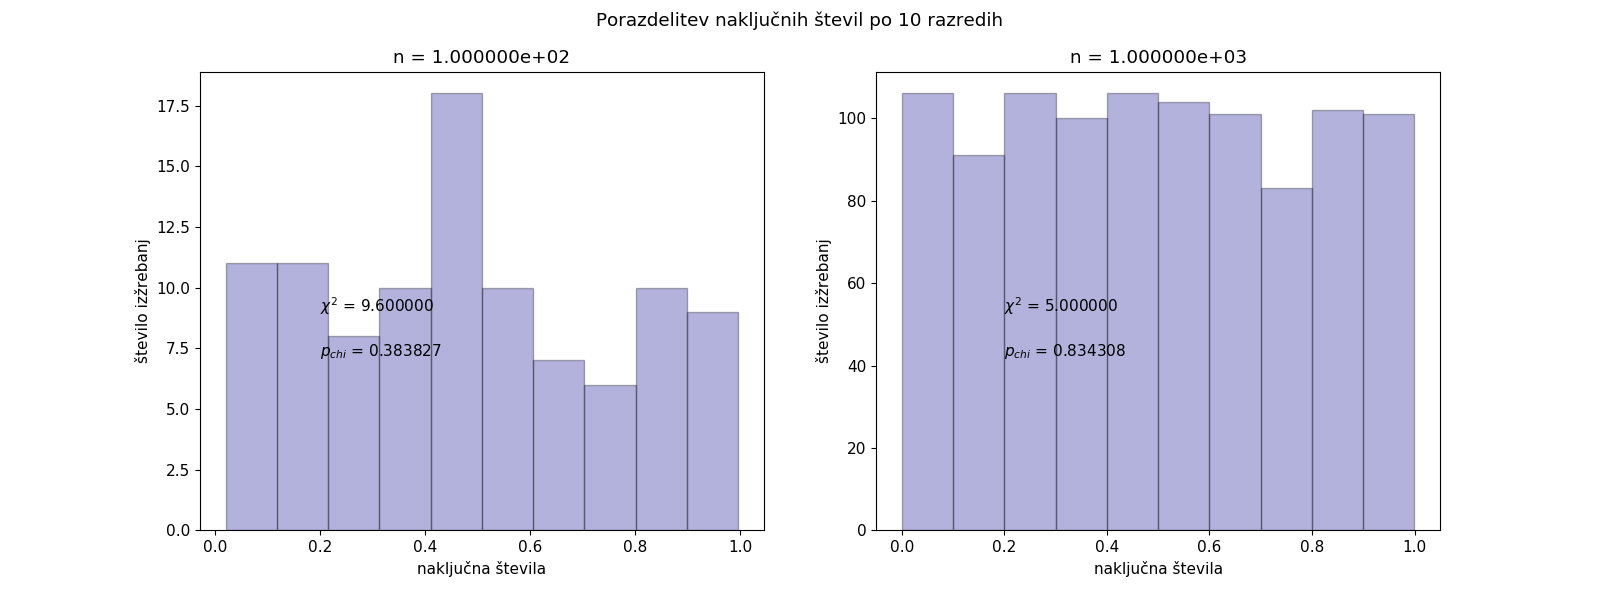
\includegraphics[width=22cm, height=6cm]{enakomerna_1.png}
 \caption{Histogram 10 razredov za različno število naključnih žrebov (n=100,1000). Vidimo, da z višanjem števil vse bolj zapolnimo prostor in imamo res enakomerno porazdelitev.}
\end{figure}
\begin{figure}[H]
\hspace*{-2.5cm}  
  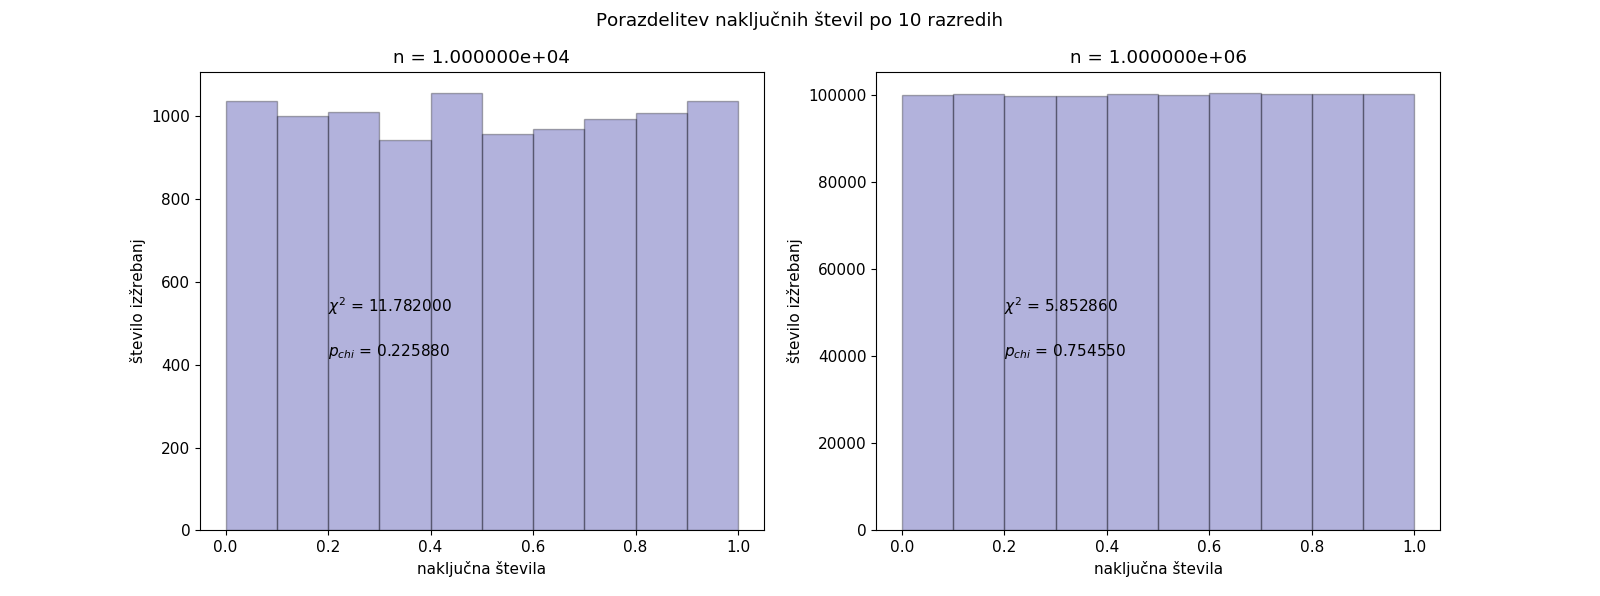
\includegraphics[width=22cm, height=6cm]{enakomerna2.png}
 \caption{Histogram 10 razredov za različno število naključnih žrebov. Vidimo, da z višanjem števil vse bolj zapolnimo prostor in imamo res enakomerno porazdelitev. Vidimo, da je za vse n zadoščen pogoj $\chi^2 < \chi_D^2$ oziroma $p > 0.05$. }
\end{figure}
Vsakič ko naključno vlečemo števila seveda $\chi^2$ ne pride isti. Porazdeljen je po analitičnem porazdelitvenem zakonu $\frac{dP}{d\chi^2}$ za $ n_{razredov} - 1 $ prostostnih stopenj. V primeru da je naša porazdelitev res enaka (ničta hipoteza H0) bodo $\chi^2$ morali nanizati porazdelitev za ustrezne prostostne stopnje.
\begin{figure}[H]
\hspace*{-2.5cm}  
  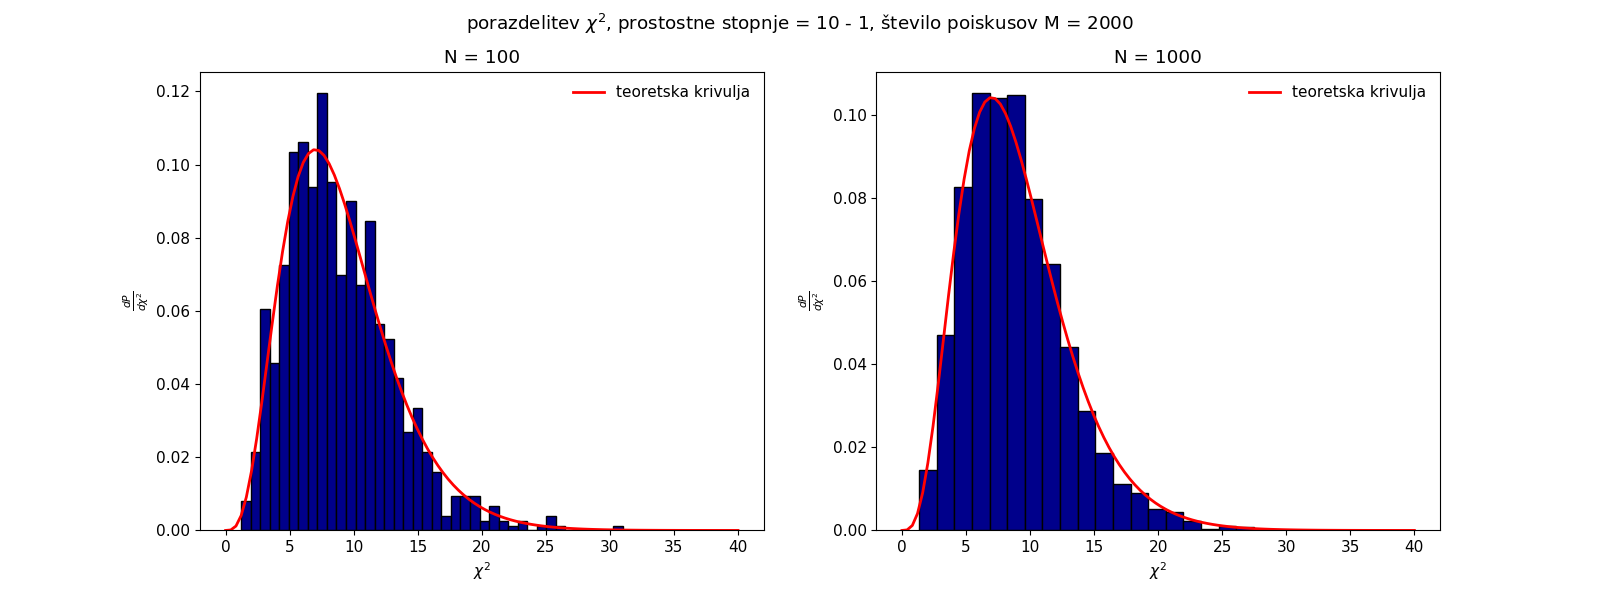
\includegraphics[width=22cm, height=6cm]{hi_statistika_1.png}
 \caption{Po 2000 poiskusih naključnega žreba 100, 1000 števil vidimo da je hi-kvadrat res porazdeljen po ustreznem zakonu s povprečjem $n_{razredov}-1$, in še en dokaz, da naša hipoteza o enakosti porazdelitev drži. }
\end{figure}
\begin{figure}[H]
\hspace*{-2.5cm}  
  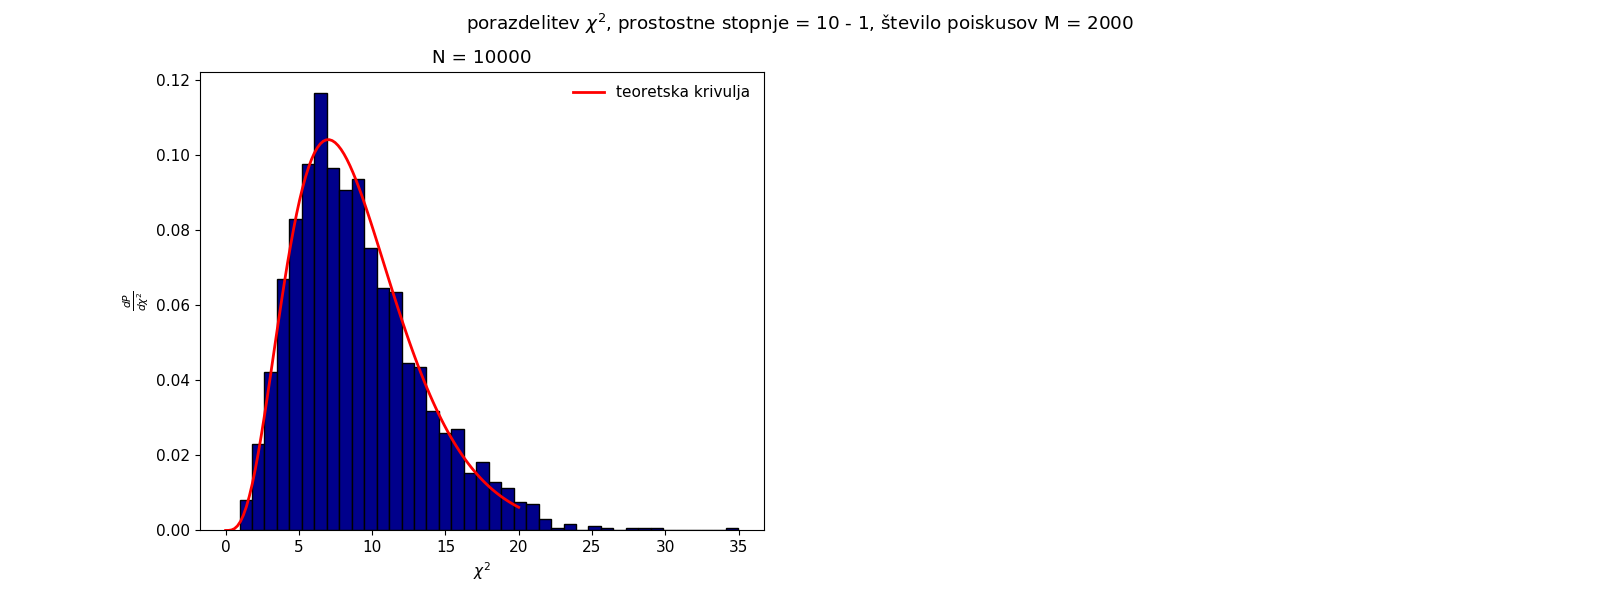
\includegraphics[width=22cm, height =6cm]{hi_statistika_2.png}
 \caption{}
\end{figure}
\subsection{Test Kolmogorov - Smirnov}
Opravimo lahko tudi test kolmogorova, kjer primerjamo dve kumulativni porazdelitvi, tako da iščemo največjo razdaljo med kumulativnima porazdelitvama
\begin{equation}
D= \sup_x |F_n(x)-F(x)|,
\end{equation}
kjer je $F_n(x)$ izmerjena kumulativna porazdelitev in $F(x)$ testna porazdelitev. Kolmogorov je dokazal, da so $D\sqrt{N}$,kjer je ($N$ število izmerkov), porazdeljeni po zakonu Kolmogorova, in zato lahko testiramo enakost porazdelitev. Če sta porazdelitvi res enaki, bodo morali biti za dane prostostne stopnje, $D\sqrt{N}$  porazdeljeni po zakonu Kolmogorova. Če pa smo porazdelitev zgrešili pa bodo $D$ veliko večji in tako ne bodo porazdeljeni po zakonu Kolmogorova za dane prostostne stopnje. To lahko zopet simuliramo s $M$ ponovitvami žrebov naključnih števil in vsakič izračunamo test Kolmogorova med žrebom in enakomerno porazdelitvijo. 
\begin{figure}[H]
\hspace*{-2.5cm}  
  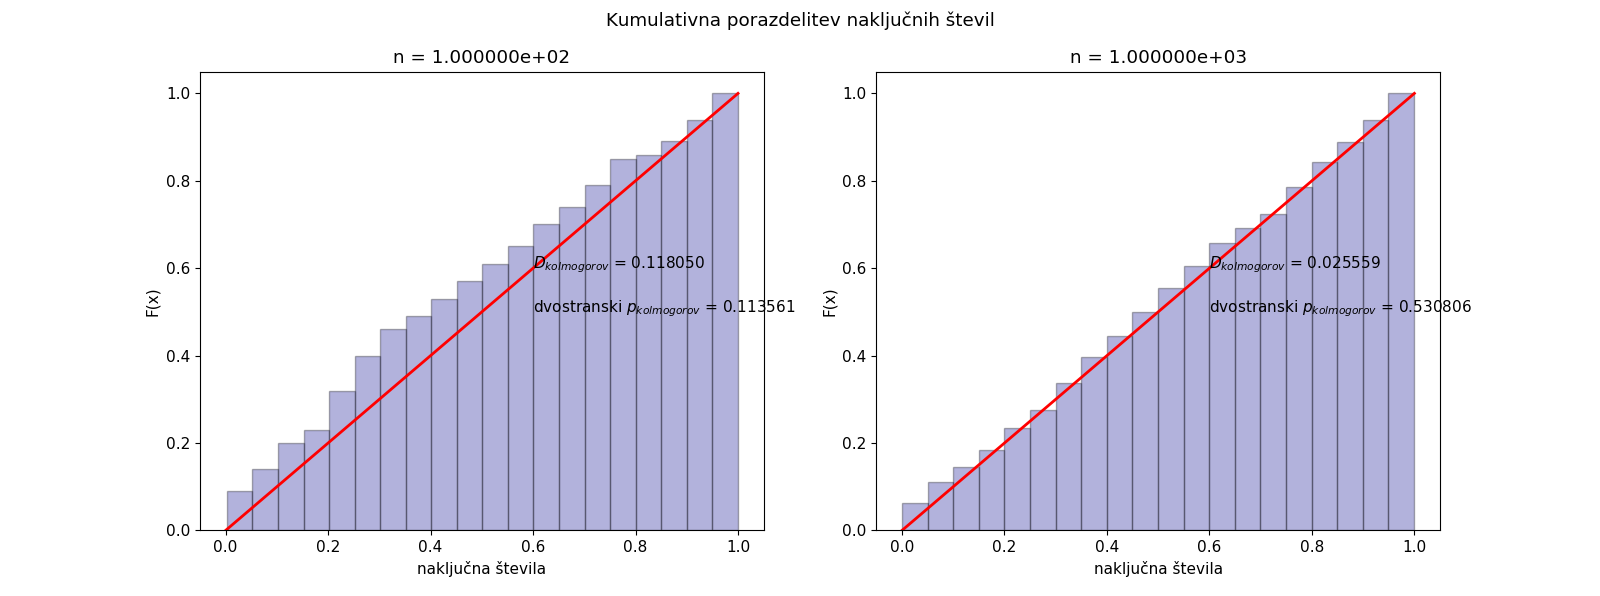
\includegraphics[width=22cm, height = 6cm]{enakomerna_kolmogorov_1.png}
 \caption{}
\end{figure}
\begin{figure}[H]
\hspace*{-2.5cm}  
  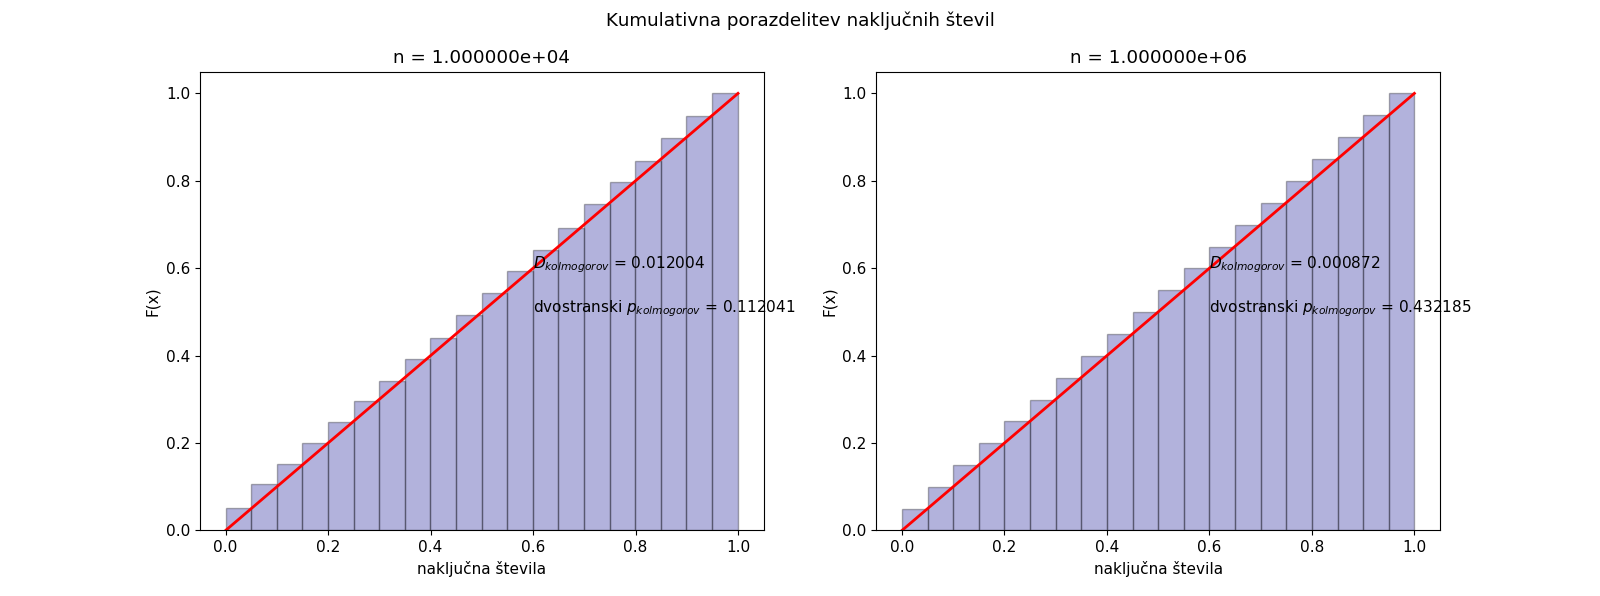
\includegraphics[width=22cm , height = 6cm]{enakomerna_kolmogorov_2.png}
 \caption{Vidimo, da je pri vseh razdalja dovolj velika, da je levo in desno od aboslutne vrendosti razdalje verjetnost $p > 0.05$. }
\end{figure}
\begin{figure}[H]
\hspace*{-2.5cm}  
  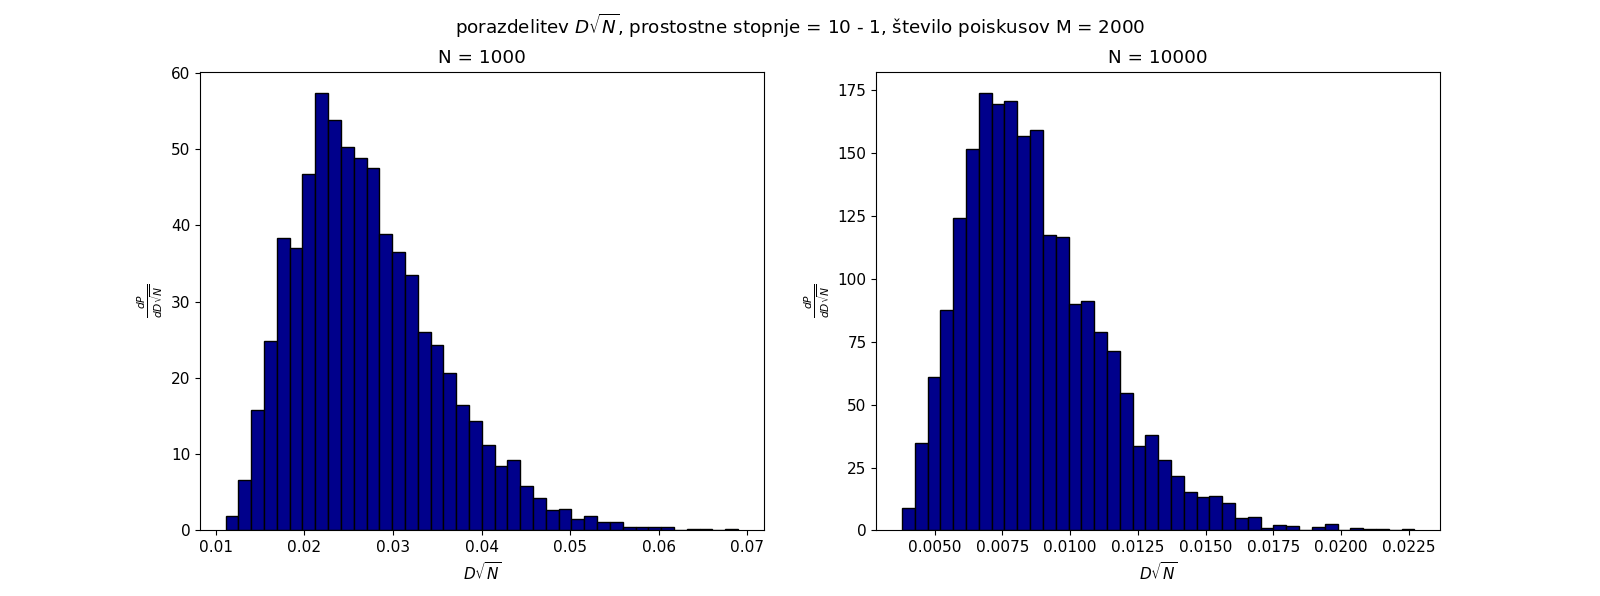
\includegraphics[width=22cm, height =6cm]{enakomerna_kolmogorov_3.png}
 \caption{Porazdelitev statistike ustreza porazdelitvi kolmogorova. }
\end{figure}

\section{Normalno porazdeljena naključna števila}
Za simulacije večinoma ne potrebujemo enakomerno porazdeljenih naključnih števil, temveč nekakšno drugo porazdelitev npr. normalno.
\subsection{Box Muller}
Box - Muller transformacija nam dve enakomerno porazdeljenih naključnih števili transformira v normalno porazdeljeni naključni števili s transformacijo.
\begin{equation}
\begin{split}
Z_1 &=R \cos(\Theta) =\sqrt{-2 \ln U_1} \cos(2 \pi U_2), \\
Z_2 &= R \sin(\Theta) = \sqrt{-2 \ln U_1} \sin(2 \pi U_2).
\end{split}
\end{equation}
Drug način pa je konvolucijski tip generatorja, kjer vzamemo konvolucijo enakmerne porazdelitve in po centralnem limitnem teoremu preidemo v normalno porazdelitev. Tako vzamemo npr. 6 naključnih števil iz random generatorja in jih seštejemo, ter nato 6 naključnih števil odštejemo, da bo normalna porazdelitev imela povprečje 0 in sigmo ena.
\begin{equation}
Z = \sum_i^6 X_i - \sum_i^6 Y_i
\end{equation}
Očitno je da je konvolucijski algoritem počasnejši saj potrebuje 6 krat več računati naključna števila kot Box Muller.
\begin{figure}[H]
\hspace*{-2.5cm}  
  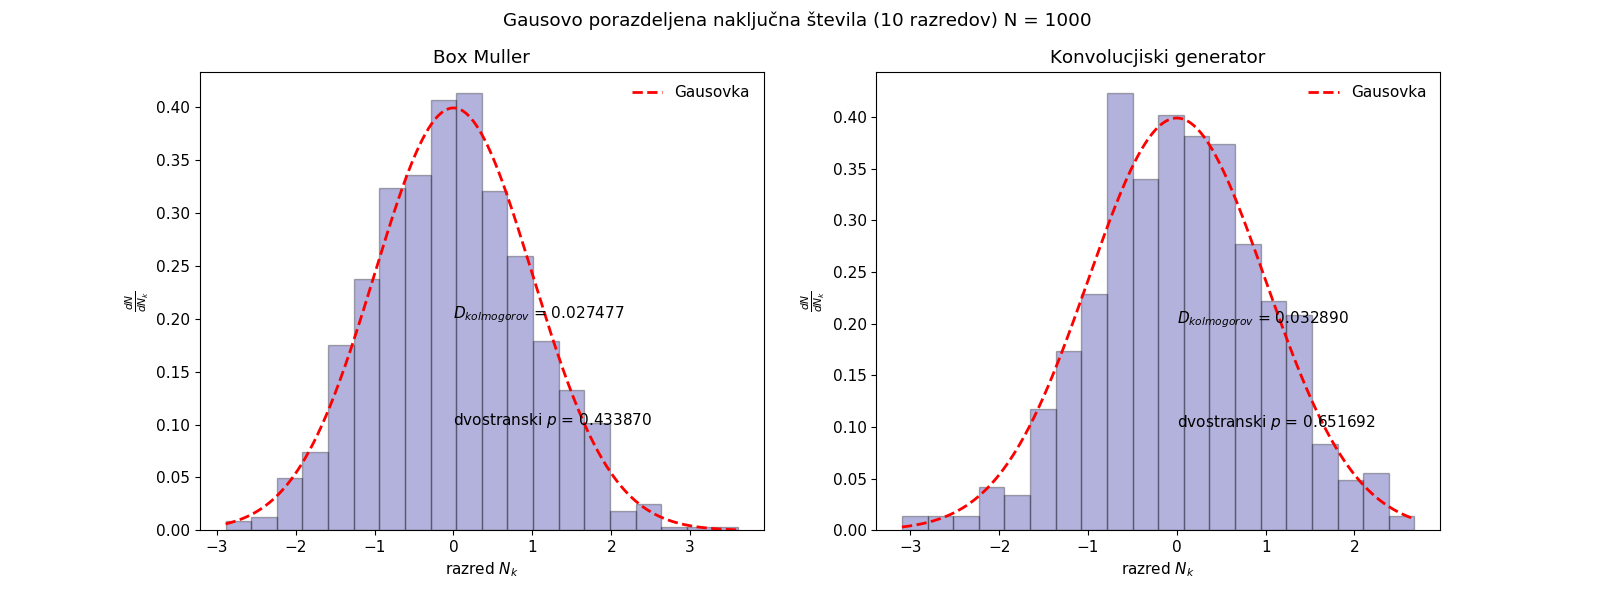
\includegraphics[width=22cm, height =6cm]{normalna_1.png}
 \caption{Naključno generirana števila (N= 1000) porazdeljena po normalni porazdelitvi. Porazdelitev smo testirali s testom Kolmogorov - Smirnov, in očitno je $p > 0.05$, torej lahko potrdimo normalno porazdelitev.  }
\end{figure}
\begin{figure}[H]
\hspace*{-2.5cm}  
  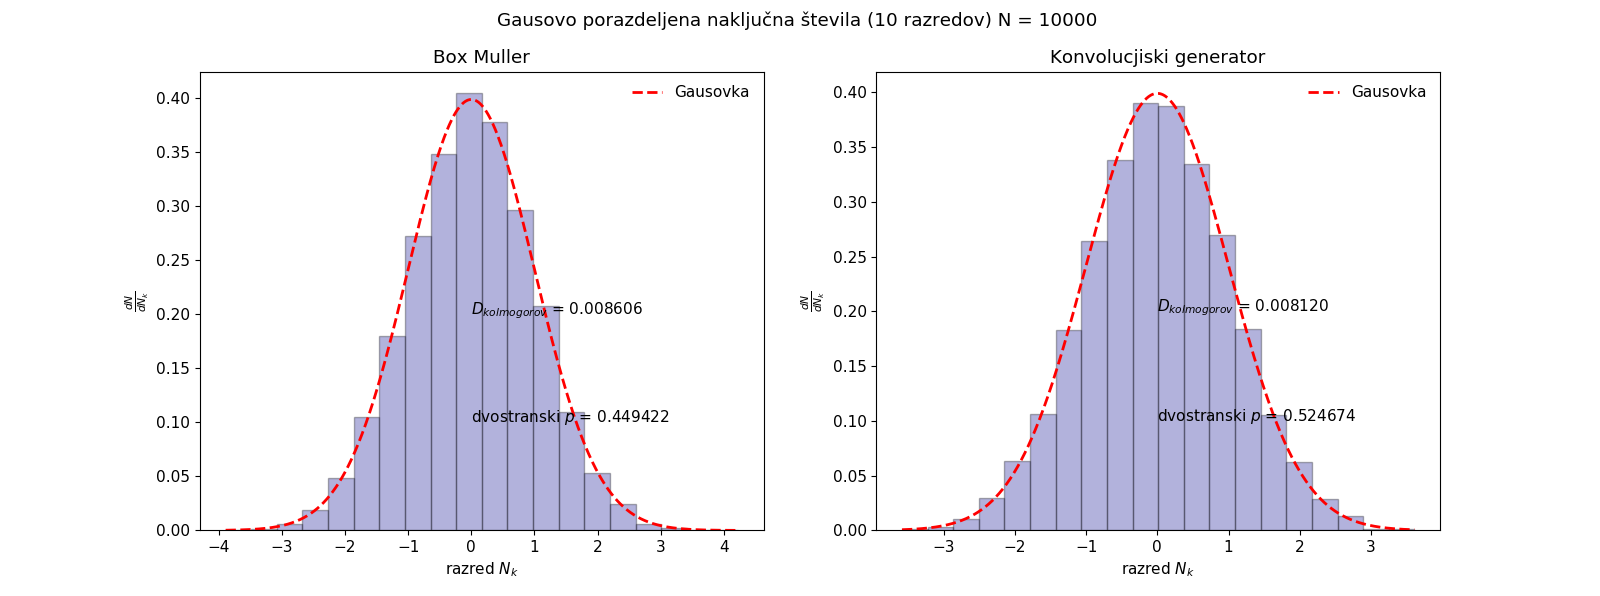
\includegraphics[width=22cm, height =6cm]{normalna_2.png}
 \caption{Naključno generirana števila (N= 10000) porazdeljena po normalni porazdelitvi. Pri višanju žrebov se razredi vse bolj polnijo in je porazdelitev vedno lepša. }
\end{figure}
Zanima nas časovna zahtevnost generatorja Box-Muller in konvolucijskega generatorja
\begin{figure}[H]
\hspace*{-2.5cm}  
  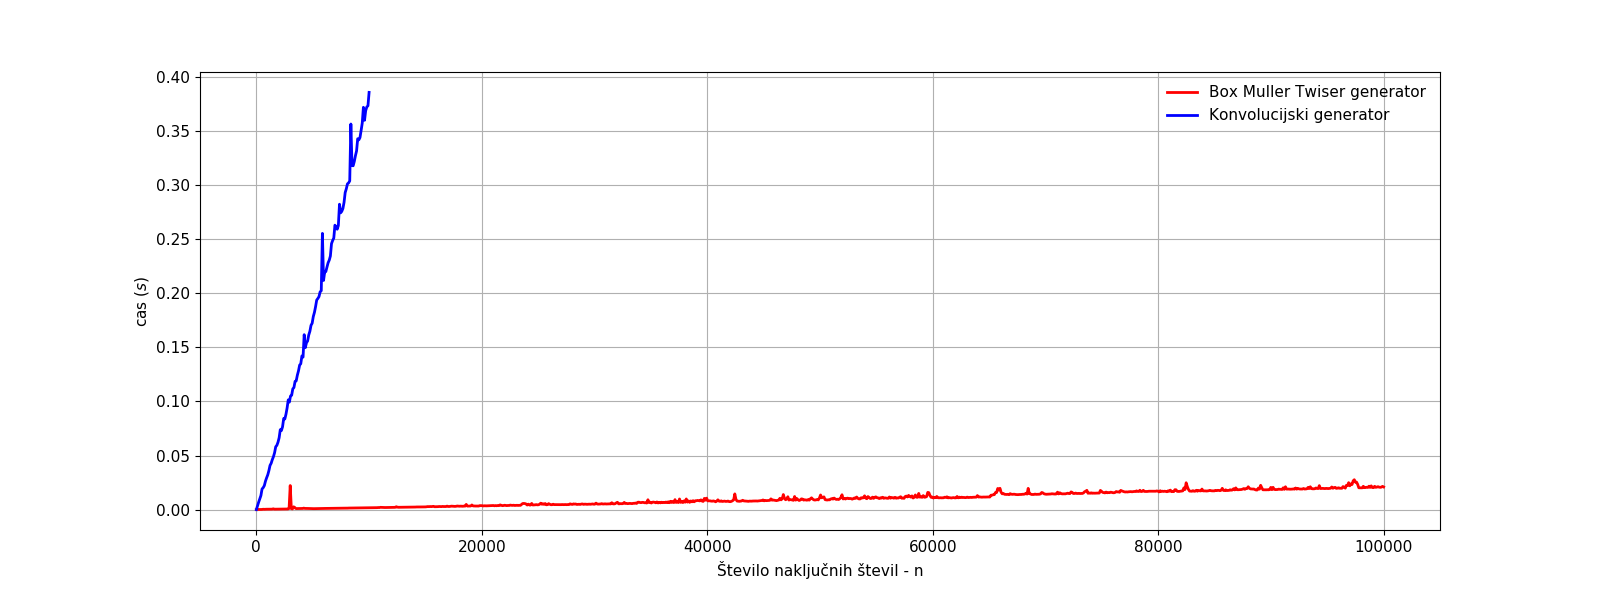
\includegraphics[width=22cm, height =6cm]{normalna_3.png}
 \caption{Vidimo, da je časovna zahtevnost gneratorja O(n), vendar pa je pri konvolucijskem generatorju premica približno šestkrat bolj strma. }
\end{figure}
\section{Porazdelitev parov naključnih števil v prostoru}
\subsection{Enakomerna porazdelitev števil}
Najprej vzemimo 2 para števil in se prepričajmo, da so pari števil naključno porazdeljeni po prostoru
\begin{figure}[H]
\hspace*{-2.5cm}  
  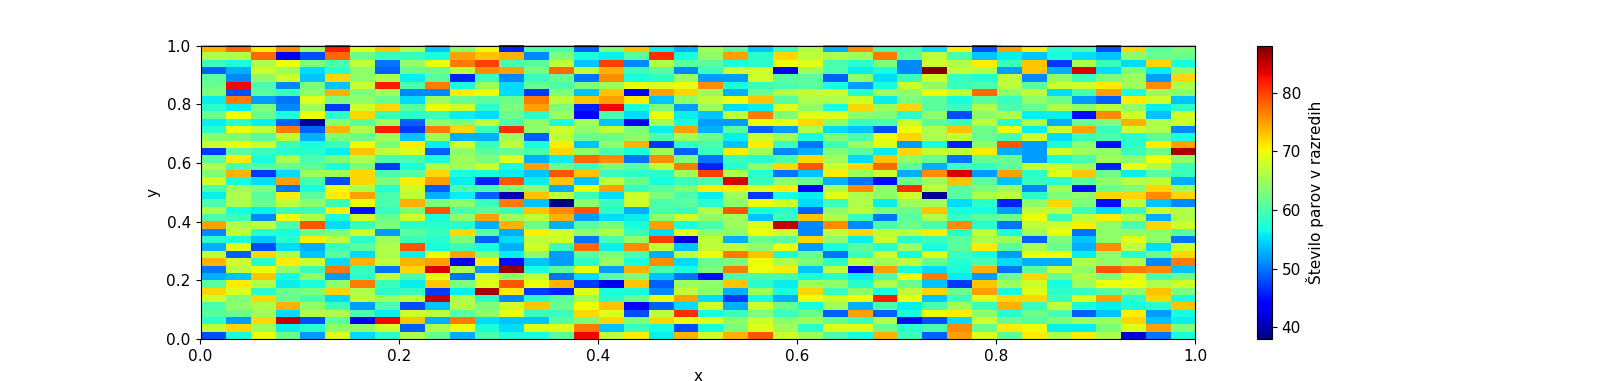
\includegraphics[width=21cm,height=6cm]{druga_1_enakomerno.png}
 \caption{Porazdelitev 1000 naključnih parov števil}
\end{figure}
Porazdelitvna funkcija je tako
\begin{equation}
\frac{dP}{du dv} = \frac{1}{S} = 1
\end{equation} 
v primeru če števila enakomerno žrebamo iz kvadrata $[0,1],[0,1]$
\subsection{Enakomerna porazdelitev po krogu}
Sedaj si poglejmo kako bi namesto kvadrata [0,1]x[0,1] dobili enakomerno porazdeljene števile po krogu. Zapišimo verjetnost, da v krogu z radijem $R$ izžrebamo en ločni element.
\begin{equation}
dP = \frac{r dr d\phi}{\pi R^2}
\end{equation} 
Ker je ta verjetnost za vse ločne elemente enaka lahko zapišemo verjetnostno porazdelitev za izžrebanje para števila na krogu na intervalu $[r , r +dr], [ \phi, \phi + d \phi ]$.
\begin{equation}
\frac{dP}{dr d\phi} = \frac{r}{\pi R^2}
\end{equation} 
Vidimo, da je porazdelitev že normirana saj velja, da je $\int_{0}^{\inf} \int_{0}^{2 \pi} \frac{dP}{dr d\phi} = 1$. Kar opazimo je, da se verjetnost z večjimi radiji mora povečati, saj so tam ločni elementi večji.\newline\newline Če naivno vzamemo dve naključni števili in zapišemo $r = u1 , \phi = 2 \pi u_2$. Privzeli smo, da za vse elemente $dr$ in $d\phi$ velja enakomerna porazdelitev in zato dobimo veliko več parov števil blizu središča.
\begin{figure}[H]
\hspace*{-2.5cm}  
\centering
  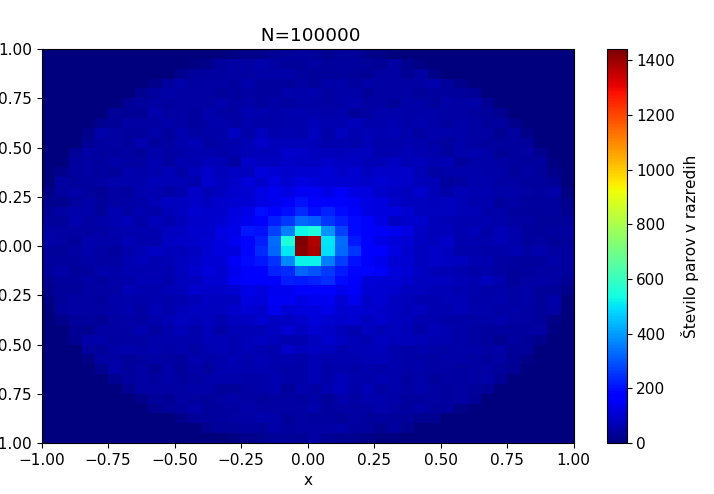
\includegraphics[width=10cm,height=6cm]{druga_narobe.png}
 \caption{Porazdelitev 10000 števil po krogu, po tem ko vzamemo r = $u_1$ in $\phi = 2 \pi u_2$, vendar pa nismo upoštevali, da ploščina ločnih elementov po krogu niso enake, kot pri enakomerni porazdelitvi temveč se večajo s radiji, zato bo tam manj števil. }
\end{figure}
Torej moramo najti pravo transformacijo iz števila $u_1,u_2 \in [0,1],[0,1] $ za kateri velja
\begin{equation}
\frac{dP}{dudv} = 1
\end{equation}
To lahko naredimo s transformacijo porazdelitev:
\begin{equation}
\frac{dP}{dudv} = \frac{dP}{dr d\phi} |\vec{J}|
\end{equation}
temu pogoju najlažje zadostimo tako, da vzamemo vsako porazdelitev posebej in zapišemo
\begin{equation}
\frac{dP}{dr} = \int_0^{2\pi} \frac{dP}{dr d\phi} =  \frac{2r}{R^2} 
\end{equation}
\begin{equation}
\frac{dP}{d \phi} = \int_0^{\inf} \frac{dP}{dr d\phi} = \int_0^{R} \frac{dP}{dr d\phi} = \frac{1}{2 \pi} 
\end{equation}
Vzemimo, da je $R=1$, sedaj lahko pogledamo kakšen mora biti $r,\phi$ da bo veljalo
\begin{equation}
\frac{dP}{du} = \frac{dP}{d r}  |\frac{dr}{du}| -> 1 = 2r |\frac{dr}{du}| -> r = \sqrt{u}
\end{equation}
\begin{equation}
\frac{dP}{d v} = \frac{dP}{d \phi }  |\frac{d \phi}{dv}| -> 1 = \frac{1}{2 \pi}|\frac{d \phi}{du}| -> \phi = 2 \phi v
\end{equation}
Če vzamemo 2 naključni števili $u_1$ in $u_2$, lahko zapišemo $r$ in $\phi$, ki sta polarni koordinati za pare števil po krogu in sta porazdeljena enakomerno po krogu s verjetnostjo  $\frac{dP}{dr d\phi} = \frac{r}{\phi}$ kar je ravno enakomerna porazdelitev.
\begin{equation}
\begin{split}
r &= \sqrt{u_1} \\
\phi &= 2 \pi u_2 \\
\end{split}
\end{equation}

\begin{figure}[H]
\hspace*{-2.5cm}  
  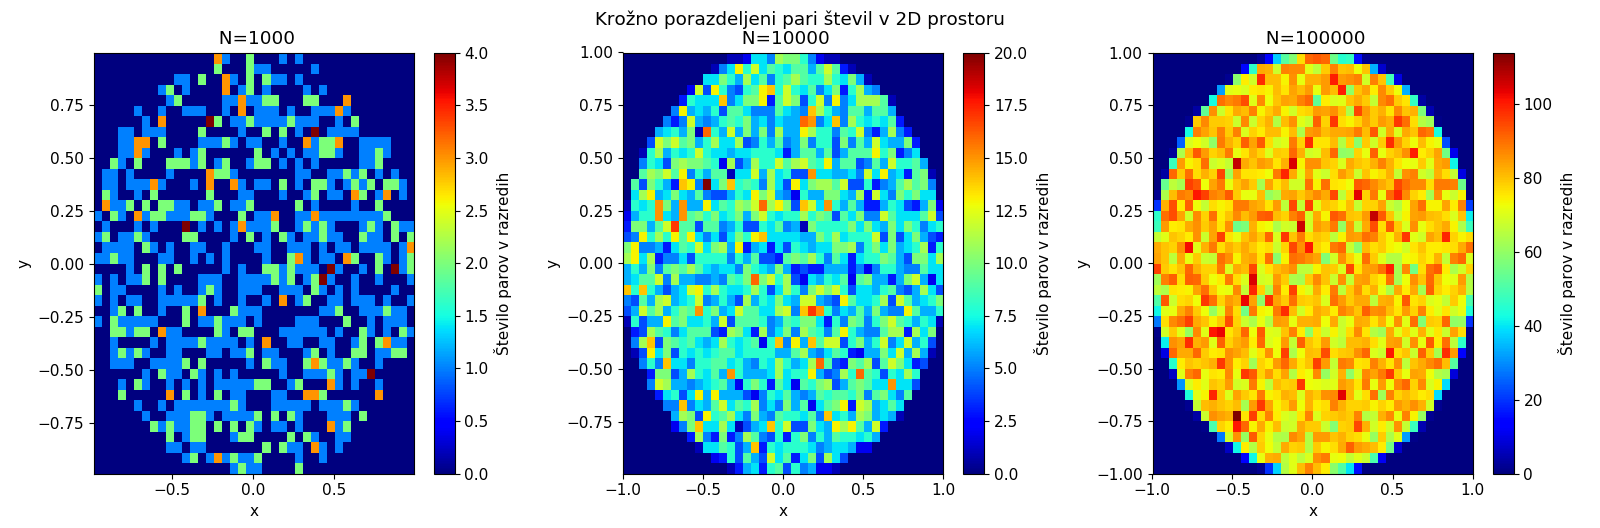
\includegraphics[width=21cm,height=6cm]{druga_1_krozno.png}
 \caption{Enakomerna porazdelitev naključnih števil po krogu je z večanjem števil vse bolj zapolnjena. Vemo da je prava porazdelitev na disku s radijem $r = 1$ enaka $f_{R \phi}(\theta)=\frac{1}{2\pi}$}
\end{figure}
S podobno transformacijo lahko transformiramo enakomerno kotno porazdelitev, ki jo prikažemo na sferi. 
\subsection{Sferična enakomerna porazdelitev}
Verjetnost da pri naključnem žrebu izberemo točko v krogli je enaka $dP  = r^2 sin ( \theta ) d \phi dr d \theta =\frac{ r^2 \phi dr d cos( \theta)} {4/3 \pi R^3} $. Torej enakomerna porazdelitev števil po krogli z radijem $R=1$ enaka 
\begin{equation}
\frac{dP}{dr d \phi  d \cos( \theta )}  = \frac{3 r^2}{4 \pi}
\end{equation} 
Torej zopet vidimo, da mora biti verjetnost pri večjih radijih večja, saj so prostorski elementi večji in jih je zato manj. Prav tako pa je verjetnost po theta odvisna od $sin(theta)$, kar pomeni, so na ekvatorju prostorski elementi prav tako manjši in je zato tam verjetnost, da smo naključno izbrali tisti prostorski element večja. \newline\newline
\textbf{Na slednjih primerih smo ugotovili, da je porazdelitev po drugih koordinatah ni konstantna tako kot v kartezičnih koordinatah, čeprav pa nam opisuje enakomerno porazdelitev elementov po krogli/krogu.}\newline\newline
\textbf{Sedaj tudi razumemo, da moramo enakomerno porazdelitev v kartezičnih koordinatah prevesti na dano porazdelitev v sferičnih koordinatah (npr. enakomerno, dipolno,...), pri tem pa moramo upoštevati Jakobijevo determinanto. Tako lahko dobimo kakšna mora biti transformacija normnalno porazdeljene spremenljivke u, da bo nova porazdelitev enaka željeni}\newline\newline
Če nas zanima samo prostorski kot je enakomerna porazdelitev po prostorskem kotu enaka 
\begin{equation}
\frac{dP}{d \phi d \cos( \theta )} = \frac{1}{4 \pi}
\end{equation}
zopet ločimo verjtnosti tako da pointegiramo po preostali koordinati in dobimo
\begin{equation}
\frac{dP}{d \phi} = \int_{-1}^{1}\frac{dP}{d \phi d \cos( \theta )} d cos( \theta) = \frac{1}{2 \pi}
\end{equation}
\begin{equation}
\frac{dP}{d cos( \theta} = \int_{0}^{2 \pi} \frac{dP}{d \phi d \cos( \theta )} d \phi = \frac{1}{2}
\end{equation}
Mi imamo na voljo enakomerno porazdeljeni dve števili $u_1,u_2$ za kateri velja $\frac{dP}{dudv} = 1$, zopet nas zanima kakšna je povezava med $\phi $ in $u$ da velja za $u$ enakomerna porazdelitev med $[0,1]$ za $\phi$ pa enakomerna porazdelitev po krogu.
\begin{equation}
\mathbf{\frac{dP}{d u} = \frac{dP}{d \phi }  |\frac{d \phi}{du}|}  \rightarrow 1 = \frac{1}{2 \pi}|\frac{d \phi}{du}| \rightarrow \phi = 2 \phi u
\end{equation} 
\begin{equation}
\mathbf{\frac{dP}{d v} = \frac{dP}{d cos \theta }  |\frac{d \phi}{dv}|}  \rightarrow 1 = \frac{1}{2}|\frac{d cos \theta}{dv}| \rightarrow cos\theta = 2v - 1
\end{equation} 
konstanta $A = -1$ poskrbi za pravilmo območje $cos \theta \in [-1,1]$, saj bi drugače prišlo območje med $[2,0]$


\begin{figure}[H]
 \hspace*{-2.5cm} 
  \begin{subfigure}[b]{0.65\textwidth}
  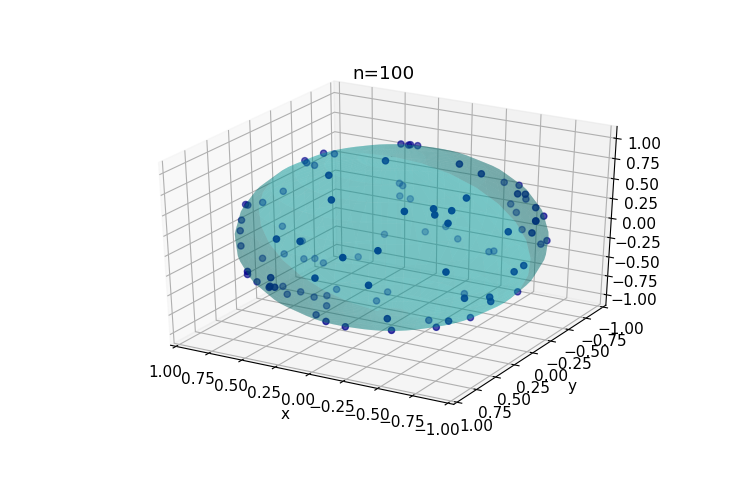
\includegraphics[width=1\textwidth, height= 6cm]{druga_krogla_1.png}
 
\end{subfigure}%
\begin{subfigure}[b]{0.65\textwidth}
  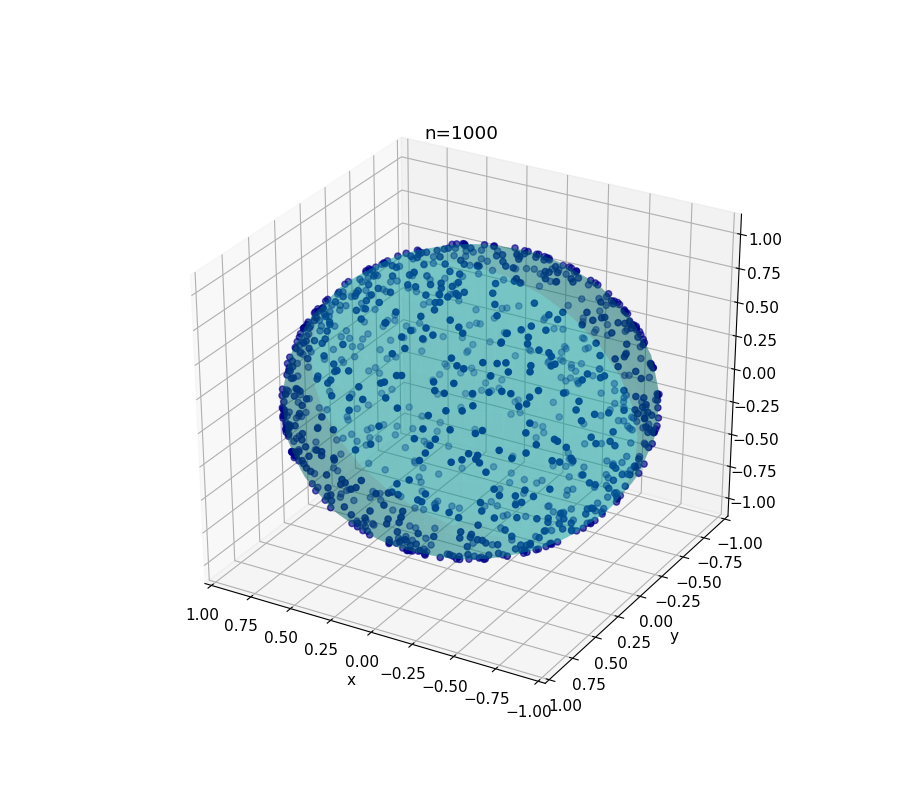
\includegraphics[width=1\textwidth, height=6cm]{druga_krogla_2.png}
 \end{subfigure}%
 
 \caption{}
\end{figure}
\begin{figure}[H]
\hspace*{-2.5cm}
\begin{subfigure}[b]{0.65\textwidth}
  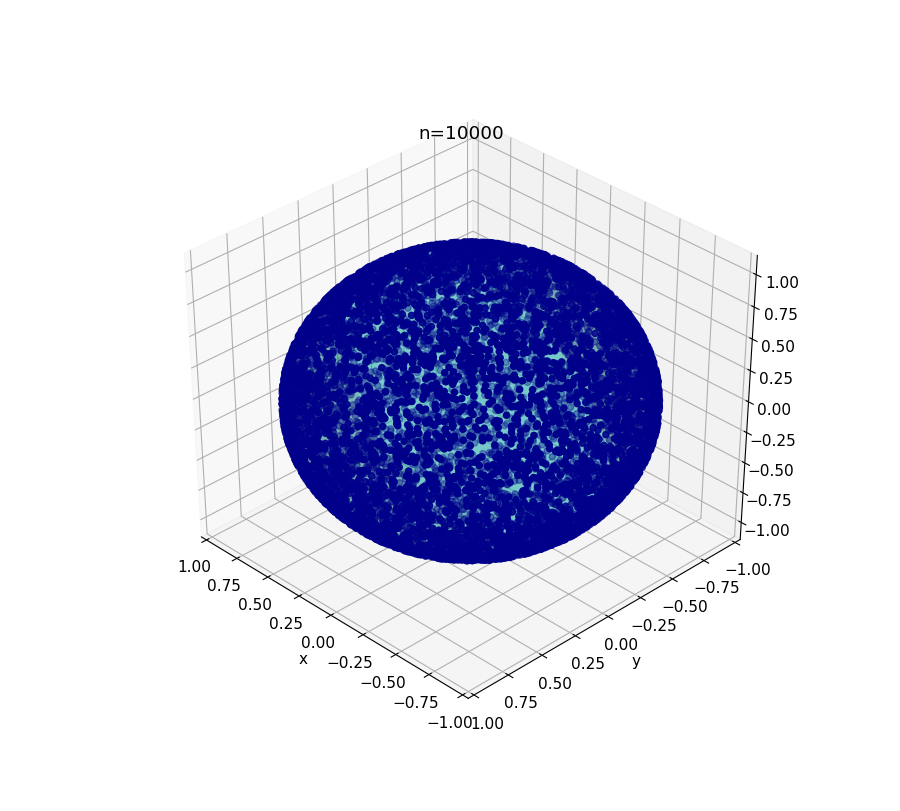
\includegraphics[width=1\textwidth, height = 6cm]{druga_krogla_3.png}
 \end{subfigure}%
 \caption{vidimo da s tako transformacijo res dobimo enakomerno porazdelitev parov števil po krogli.} 

\end{figure} 
Poglejmo si še povprečne vrednosti različnih momentov
\begin{table} [H]

\label{my-label}
\begin{tabular}{lllllll}
\centering
N & $<\theta$> & $\sigma^2_{\theta}$ & $<\phi>$ & $\sigma^2_{\phi}$ & $\langle\cos{\theta}\rangle$ & $\sigma^2_{\langle\cos{\theta}\rangle}$ \\
100 & 1.5742 & 0.1051 & 3.2121 & 0.1215 & -0.0043 & 0.04 \\
1000 & 1.5641 & 0.0152 & 3.1321 & 0.0566 & -0.0126 & 0.0043 \\
10000 & 1.5712 & 0.0071 & 3.1321 & 0.0114 & -0.0012 & 0.001 
\end{tabular}
\end{table}
Vidimo, da se momenti ujemajo s teoretičnimi vrednostmi, torej povprečni $\phi = \pi$, povprečna $\theta = \frac{\pi}{2}$ in povprečni $cos \theta = 0$.
Vrednosti $\theta$ se po pričakovanjih gibljejo okoli $\pi/2$, vrednosti $\phi$ okoli $\pi$, $\langle\cos{\theta}\rangle$ pa okoli ničle. 

\subsection{Dipolna porazdelitev naključnih števil}
Sedaj pa nas namesto enakmoerne porazdelitve števil po krogli zanima kakšna druga porazdelitev, npr. porzadelitev dipolnega sevanja, ki je  sorazmerna s $sin^2 \theta$. Vemo, da je porazdelitev enaka
\begin{equation}
\frac{dP}{d \Omega}  = A sin^2 ( \theta) = \frac{3}{8 \pi} sin^2( \theta)
\end{equation}
Izverednotimo sedaj porazdelitev po vsakem kotu posebej.
\begin{equation}
\begin{split}
\frac{dP}{d cos\theta} &= \frac{3}{4} sin^2( \theta) \\
\frac{dP}{ d \phi } &= \frac{1}{2 \pi} 
\end{split}
\end{equation}
Zanima nas zopet kako zagotoviti, da enakomerna porazdelitev med $[0,1]$ po $u$ pri transformaciji iz $u \rightarrow \theta$ pridelala dipolno porazdelitev , tako da za porazdelitveno funkcijo, da velja $\frac{dP}{du} = \frac{ dP} {d cos \theta} | \frac{ d \cos \theta} {du} |$.
\begin{equation}
1 = \frac{3}{4} sin^2( \theta) | \frac{ d \cos \theta} {du} | 
\end{equation}
\begin{equation}
du = \frac{3}{4} sin^2( \theta) d cos \theta
\end{equation}
\begin{equation}
u = \frac{1}{4} (3 cos \theta - cos^3 \theta) + \frac{1}{2} 
\end{equation}
$ A = \frac{1}{2}$ da velja $u \in [0,1]$. Te enačbe ne moremo obrniti zato moramo problem rešiti numerično. Za vsak u moramo najti ustrezen $\cos \theta$. Če bomo sedaj tako naključno izžrebali števila in izračunali vsakič $\cos \theta$, ki zadošča enačbi (25) bi morala naša porazdelitev ustrezati dipolnem sevanju. Po $\phi$ pa je transformacija enaka kot pri enakomerni porazdelitvi pri krogli, torej $\phi = 2 \pi v$.
\subsection{Numerično reševanje transformacijske enačbe}
Enačbo (25) rešujmo numerično s iteracijskimi metodami (newtnova, sekantna), bisekcijo, ali pa uporabimo $python fsolve$. Sam sem uporabil slednjo in za $N= 10000$ naključnih števil med $[0,1]$ izračunal ustrezne $\theta$.
\begin{figure}[H]
\hspace*{-2.5cm}  
  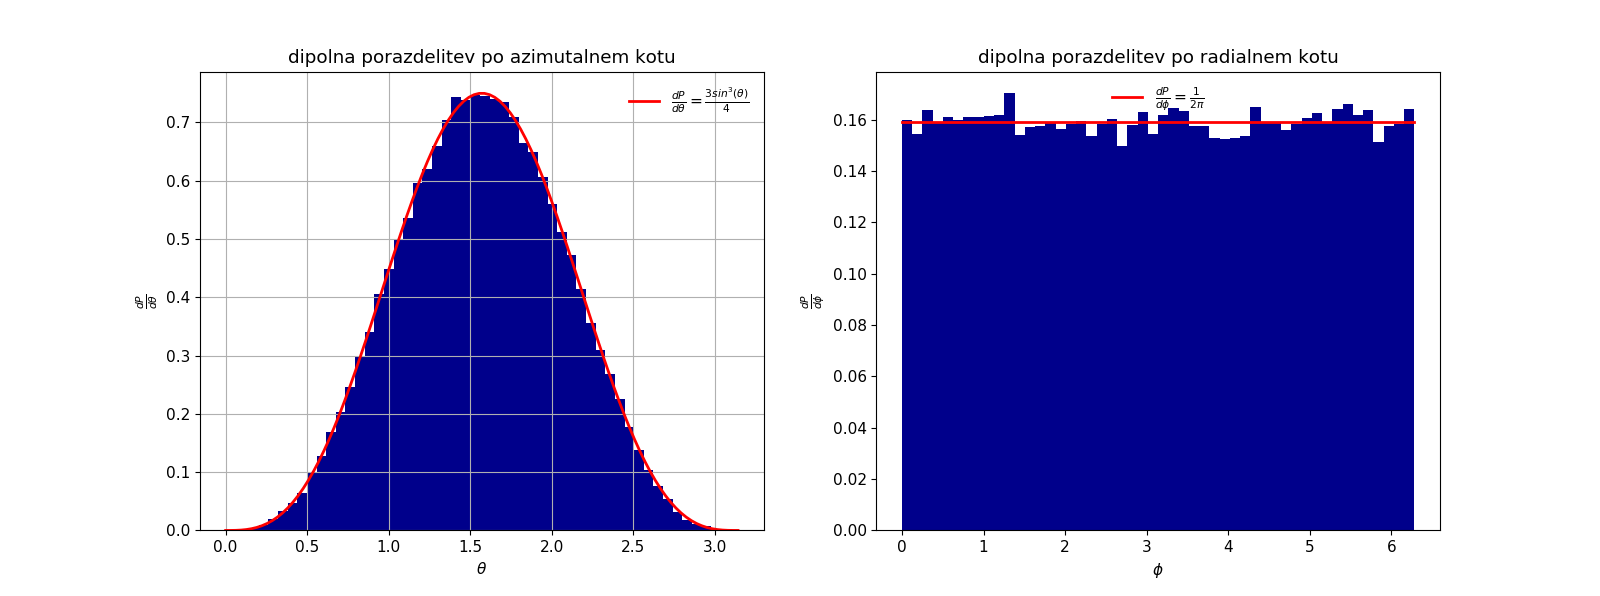
\includegraphics[width=22cm,height=6cm]{druga_dipolno1.png}
  \caption{Porazdelitev dipolnega sevanja po kotu $\phi$ in $\theta$}
\end{figure}

\begin{figure}[H]
\hspace*{-2.5cm}  
\centering
  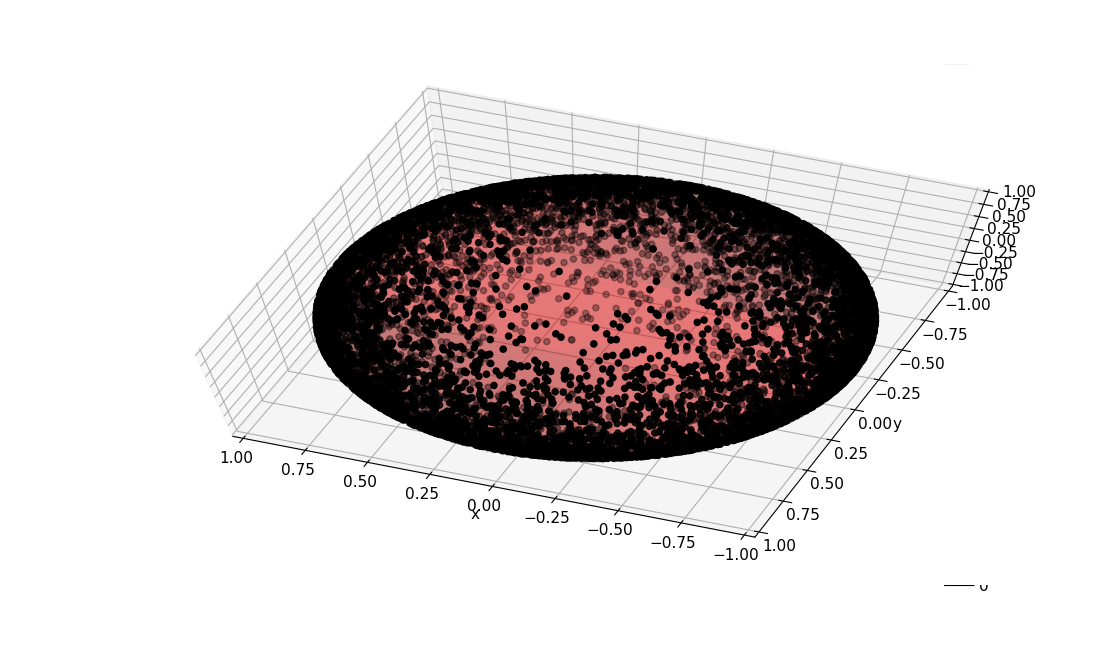
\includegraphics[width=13cm,height=6cm]{druga_dipolno.png}
  \caption{Porazdelitev na krogli vidimo, da dipol seva le v eni smeri. V našem primeru torej sumimo, da je dipol usmerjen v smeri z, saj je sevanje pravokotno iz njega najmočnejše.} 
\end{figure}
Poglejmo si še momente in jih preverimo s teoretičnimi 
\begin{table}[H]
\centering
\caption{Vrednosti povprečnega $\theta$, $\phi$, $\cos{\theta}$, $\cos^2{\theta}$ in njihovih varianc za različne $N$}
\label{my-label}
\begin{tabular}{lllllllll}
N & $<\theta$> & $\sigma^2_{\theta}$ & $<\phi>$ & $\sigma^2_{\phi}$ & $\langle\cos{\theta}\rangle$ & $\sigma^2_{\langle\cos{\theta}\rangle}$ & $\langle\cos^2{\theta}\rangle$ & $\sigma^2_{\langle\cos^2{\theta}\rangle}$ \\

1000 & 1.5821& 0.011& 3.15345 & 0.0744 & -0.0007& 0.0014 & 0.1769& 0.0033 \\
10000 & 1.5677 & 0.0023 & 3.1413 & 0.0112 & 0.0011 & 0.0004 & 0.2041 & 0.0012
\end{tabular}
\end{table}
Tudi tu momenti ustrezajo teoretičnim.
\section{Statistika oddaje domačih nalog iz Modelske Analize I}
Na voljo imamo podatke o oddaji modelskih nalog za leta 2010/11,2011/12,2012/13,2014/15. Iz nje lahko naredimo statistično obdelavo in najdemo razlike med letniki in nalogami.
Poglejmo si najprej razlike v oddaji med generacijami. 
\begin{figure}[H]
\hspace*{-2.5cm}  
  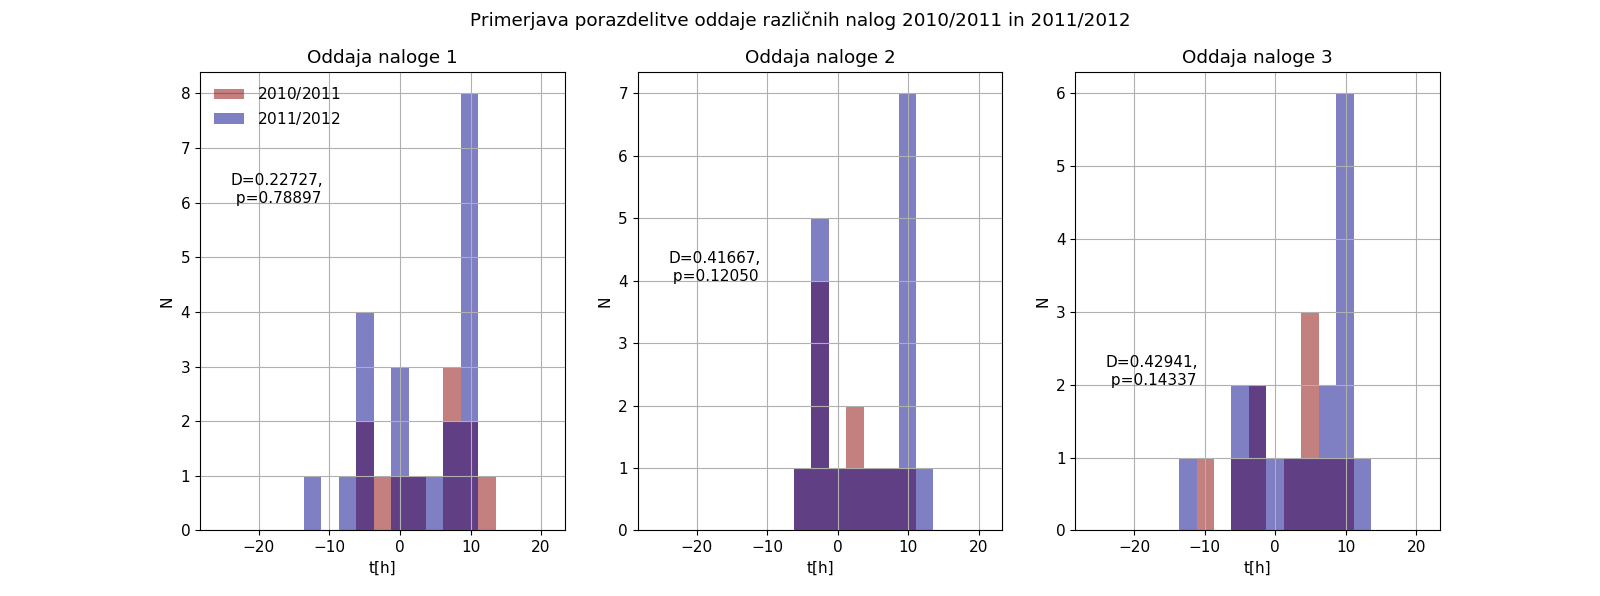
\includegraphics[width=22cm,height=6cm]{tretja_primerjava1011.png}
\end{figure}

\begin{figure}[H]
\hspace*{-2.5cm}  
  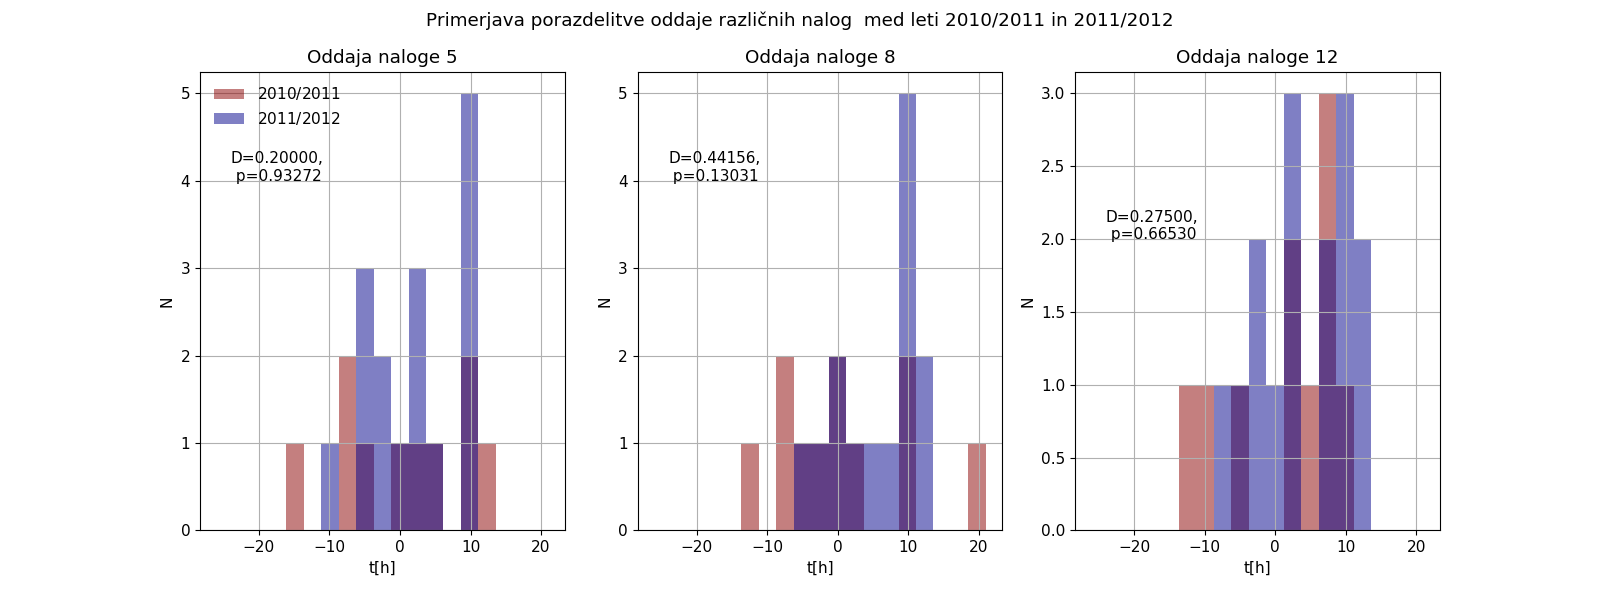
\includegraphics[width=22cm,height=6cm]{tretja_primerjava1011b.png}
 
\end{figure}
\begin{figure}[H]
\hspace*{-2.5cm}  
  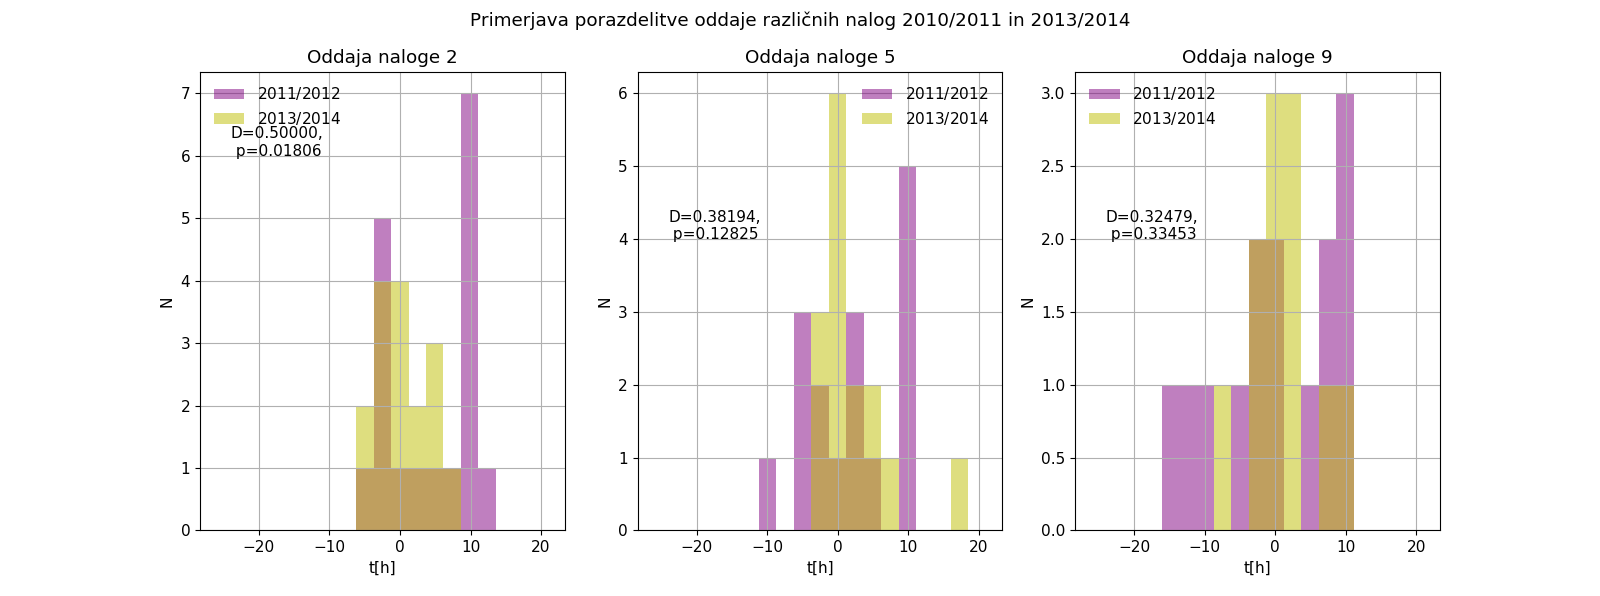
\includegraphics[width=22cm,height=6cm]{tretja_primerjava1013.png}
 
\end{figure}
\begin{figure}[H]
\hspace*{-2.5cm}  
  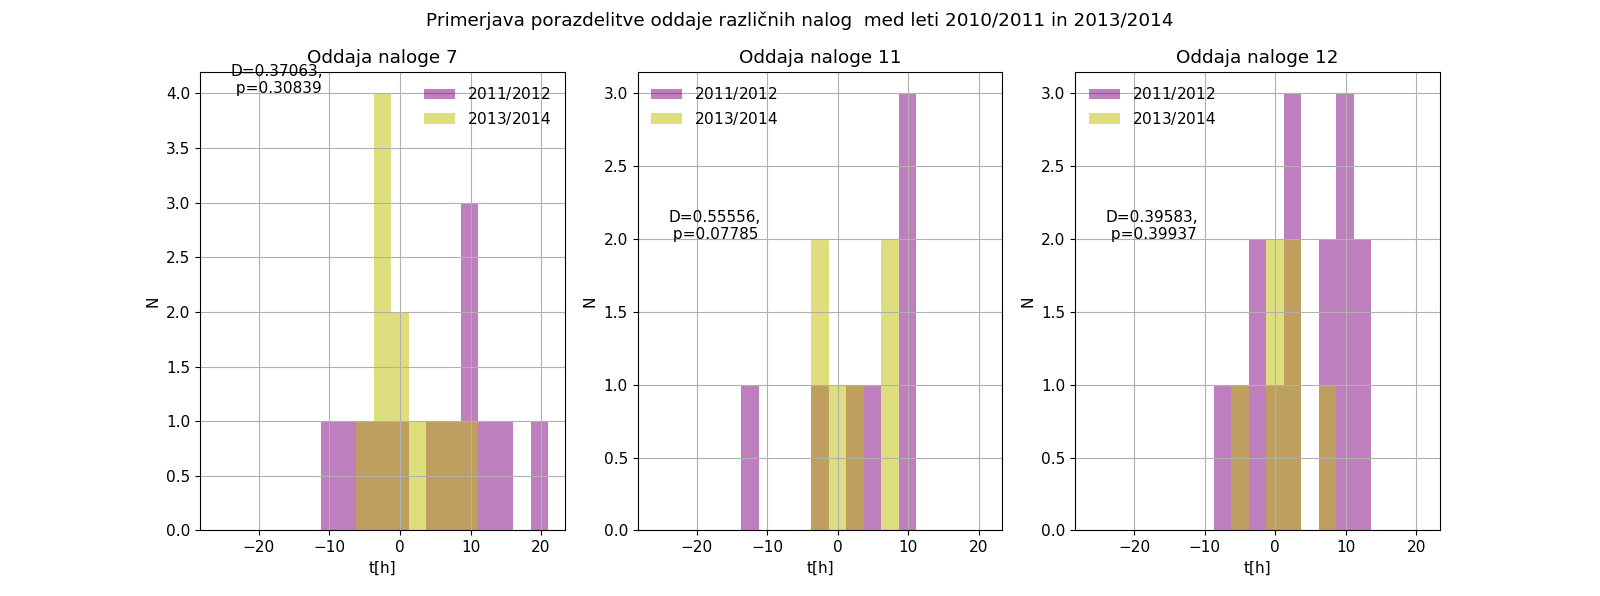
\includegraphics[width=22cm,height=6cm]{tretja_primerjava1013b.png}
 
\end{figure}
Enakost porazdelitev testiramo s testom Kolmogorov - Smirnov, in ugotovimo da razlike v oddaji nalog so (npr 11 naloga med letoma 2010/11 in 2013/14 ter 2 naloga med letom 2010/2013), kar lahko tudi vidimo, saj je bila generacija 2013/14 veliko bolj pridna, kot generacija 2010/12. 
\subsection{Primerjava oddaj različnih nalog znotraj iste generacije}
\begin{figure}[H]
\hspace*{-2.5cm}  
  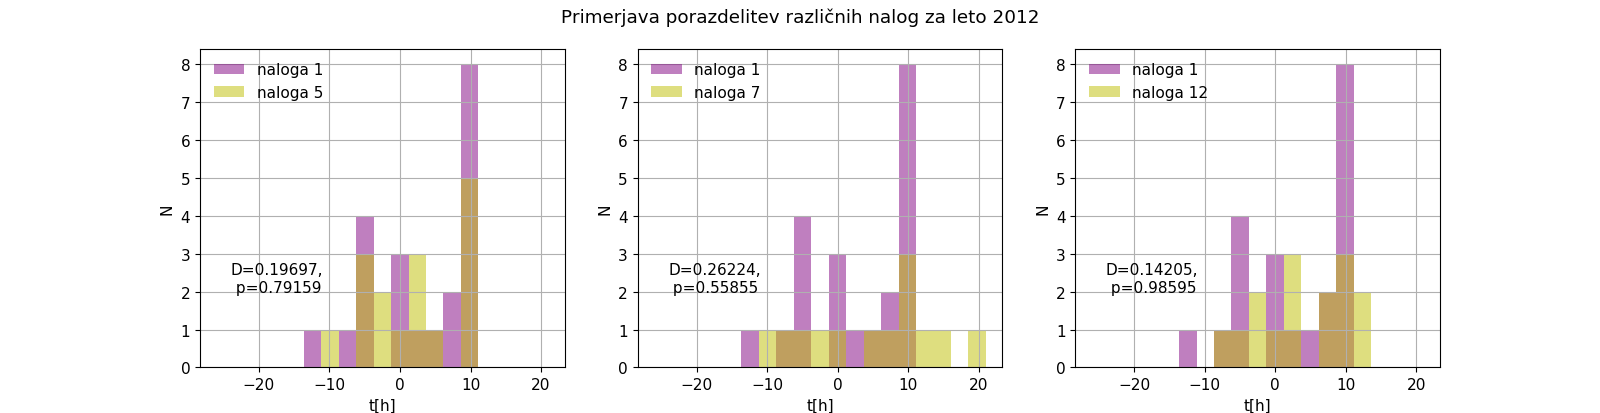
\includegraphics[width=22cm,height=6cm]{tretja_primerjava_2012.png}
 
\end{figure}
\begin{figure}[H]
\hspace*{-2.5cm}  
  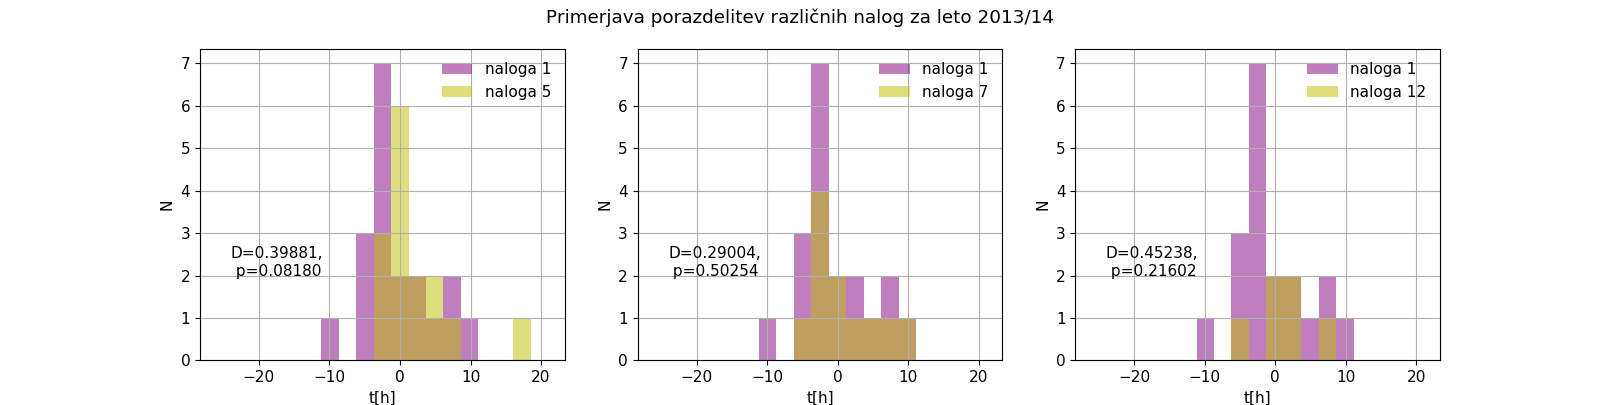
\includegraphics[width=22cm,height=6cm]{tretja_primerjava_2013.png}
  \caption{vidimo, da se znotraj generacije porazdelitve nalog razlikujejo, prav tako se močno razlikuje število, vendar pa v danih primerih ne moremo govoriti o statistično pomembni razliki med porazdlitvami naloge 1,5 ; 1,7 in 1,12. Verjetno je med kakim drugim datummom sigurno statistična pomembna razlika}
 
\end{figure}


Zanimivi so grafi kumulativne porazdelitve oddaje nalog
\begin{figure}[H]
 \hspace*{-2.5cm} 
  \begin{subfigure}[b]{0.65\textwidth}
  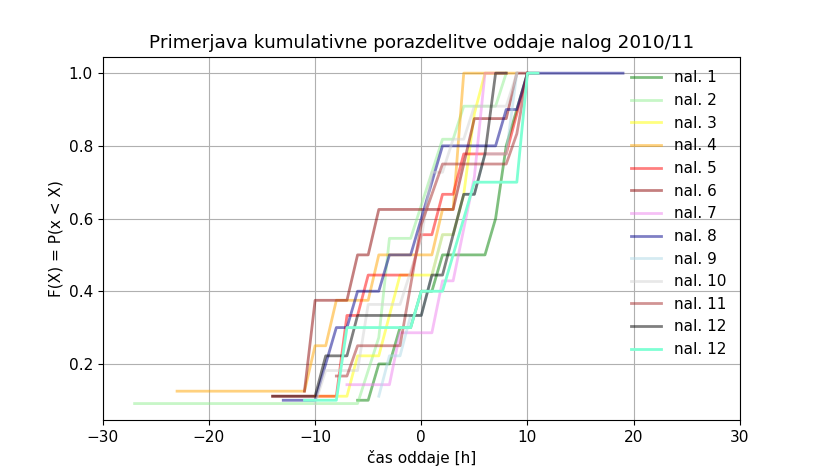
\includegraphics[width=1\textwidth]{tretja_primerjava_kumulativna1.png}
 
\end{subfigure}%
\begin{subfigure}[b]{0.65\textwidth}
  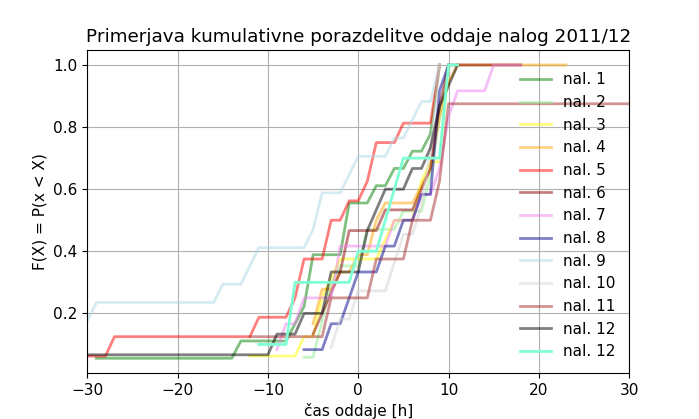
\includegraphics[width=1\textwidth]{tretja_primerjava_kumulativna2.png}
 \end{subfigure}%
 \caption{Vidimo, je ob času četrtek 00:00 oddana le polovica vseh nalog. Iz slednjega grafa se da razbrati tudi "outlinerje", kot npr. zadnja naloga 12. pri letu 2010/11 in npr. naloga 7, katero je veliko ljudi ponoči nekaj ur prepozno in npr. naloga 11 generacije 2011/12.}
\end{figure}

\section{Zaključek}

Pogledali smo si kako delujejo generatorji naključnih števil in kako iz enakomerne porazdelitve dobiti katero koli porazdelitev. Statistične porazdelitve smo testitrali s testi.
\end{document}